\documentclass{standalone}
\begin{document} 

Rechenregeln:
\begin{itemize}
    \item $x,y \in \mathbb{R}$: $x < $ ist strikt (stärker), $ x \leq y$ ist nicht strikt (schwächer) - Ungleichungen
    \item $a < b$ und $c \in \mathbb{R} \rightarrow a+c < b+c$ 
    \item $a < b$ und $c > 0 \rightarrow ac < bc$
    \item $a<b$ und $c<0 \rightarrow ac > bc$
    \item $a<b$ und $b+d \rightarrow a+c < b+d$
    \item $0<a<b$ und $0<c<d \rightarrow ac < bd$
    \item Für $a,b > 0$: $a^2 < b^2$
    \item Für $a,b > 0$: $a<b \leftrightarrow \frac{1}{b} < \frac{1}{a}$
\end{itemize}

Lösung von Ungleichungen:
\begin{itemize}
    \item Grafische Lösung durch plotten von Funktionen möglich - aber ungenau
    \item Mathematische Umformung von Ungleichung nach gesuchter Variablen
\end{itemize}
Einfaches Beispiel:
\begin{align}
    5x -4 &< 3x-1 \\
    2x &< 3 \\
    x &< \frac{3}{2}
\end{align}

Beispiel mit rationaler Funktion:
\begin{align}
    \frac{2-3x}{4x-7} &<1 \\
    \text{für } 4x-7 > 0 &\vee 4x-7 < 0 \\
    & \\
    2-3x < 4x-7 &\vee 2-3x > 4x-7 \\
    9 < 7x &\vee 9 > 7x \\
    x > \frac{9}{7}  &\vee x < \frac{9}{7}
\end{align}

Für beide Fälle müssen die Definitionsbereiche von x berücksichtigt werden. Es kann sein, dass sich die Bereiche der Fallunterscheidung und die Bereiche der Lösungen der Ungleichungen überschneiden. Die Ergebnismenge muss zu beiden kongruent sein.
\begin{itemize}
    \item Da $\frac{7}{4} > \frac{9}{7}$ gilt für Fall 1: $\mathbb{L}_1=]\frac{7}{4},+\infty[$
    \item Da $\frac{7}{4} > \frac{9}{7}$ gilt für Fall 2: $\mathbb{L}_2=]-\infty, \frac{9}{7}[$
    \item $\mathbb{L} = \mathbb{L}_1 \cup \mathbb{L}_2$
\end{itemize}

Rechenregeln für Beträge:
\begin{align}
    a &\leq \abs{a} \\
    \abs{a+b} &\leq \abs{a} + \abs{b} \\
    \abs{a-b} &\leq \abs{a} + \abs{b} \\
    \abs{\abs{a} - \abs{b}} &\leq \abs{a+b} \\
    \abs{\abs{a} - \abs{b}} &\leq \abs{a-b} \\
    \abs{ab} &= \abs{a} \abs{b} \\
    \abs{ab} &= \frac{\abs{a}}{\abs{b}}\text{, für } b \neq 0
\end{align}

Ungleichungen mit Beträgen lösen:
\begin{align}
    \abs{x-3} &\leq 2 \\
    \text{für } x-3 > 0 &\vee x-3 \leq 0 \\
    \abs{x-3} = x-3 &\vee \abs{x-3} = 3-x \\
    x-3 \leq 2 &\vee 3-x \leq 2 \\
    x \leq 5 &\vee x \geq 1 \\
    \mathbb{L}_1 = ]3, 5] &\vee \mathbb{L}_2 = [1, 3] \\
    \mathbb{L} = \mathbb{L}_1 \cup \mathbb{L}_2 = [1,5]
\end{align}

Halbebenen sind lineare Ungleichungen mit zwei Parametern, die zu einer linearen Gleichung umgeformt werden.\\
Beispiel:
\begin{align}
    x +2y &\leq 7 \\
    y &\leq -\frac{x}{2} + \frac{7}{2}
\end{align}

Zur Verifizierung von Ungleichungen können diese auf eine einfachere Form heruntergebrochen werden.
Z. B. können die Ungleichungsgesetze von oben auf beide Seiten angewandt werden (links ist a, rechts ist b).\\
Beispiel:
\begin{align}
    \sqrt{ab} &\leq \frac{a+b}{2} \\
    ab &\leq (\frac{a+b}{2})^2 \text{, mit } a^2 \leq b^2\\
    0 &\leq (a-b)^2 \text{, das ist wahr}
\end{align}
Immer nur äquivalente Umformungen machen, die das Ungleichheitszeichen stets erhalten.

\begin{align}
    b,d > 0 \text{ und } \frac{a}{b} < \frac{c}{d} \\
    \frac{a+c}{b+d} &< \frac{c}{d} \\
    ad + cd &< cb + cd \\
    ad &< cb \\
    \frac{a}{b}&<\frac{c}{d}\text{, das ist wahr}
\end{align}

Wir können Abweichungen bzw. Fehler durch den Mittelwertsatz abschätzen.
$$\abs{f(x) - f(x_0)}=\abs{f'(\xi)}\abs{x-x_0}$$
Dabei liegt $\xi$ zwischen Zielpunkt $x_0$ und Istpunkt $x$. \\
Wir nehmen eine Ansetzgenauigkeit an, sodass $\abs{x-x_0} \leq \epsilon$.
Der Maximalwert von $f'(x)$ ist gesucht, da die maximale Abweichung bereits eingeschränkt ist.
Wenn eine Funktion $f(x)$ vorliegt, sowie Abschätzungen von $\epsilon$, so kann der Maximalwert der Steigung auf dem Intervall berechnet werden.

\begin{align}
    \abs{f(x) - f(x_0)} = \abs{f'(\xi)}\abs{x-x_0} \leq M\cdot\epsilon \text{, mit } f'(\xi) \leq M \text{ und } \abs{x-x_0} \leq \epsilon \\
    M=\underset{y \in [x_0 - \epsilon, x_0 + \epsilon]} f'(x)
\end{align}

\subsection{Aufgabe 4.9}

\begin{enumerate}[a)]
    \item $M_1 = \{ (x,y)^T \in \mathbb{R}^2 \mid \abs{x} + \abs{y} \leq 1 \}$
    \begin{figure}[htbp]
        \centering
        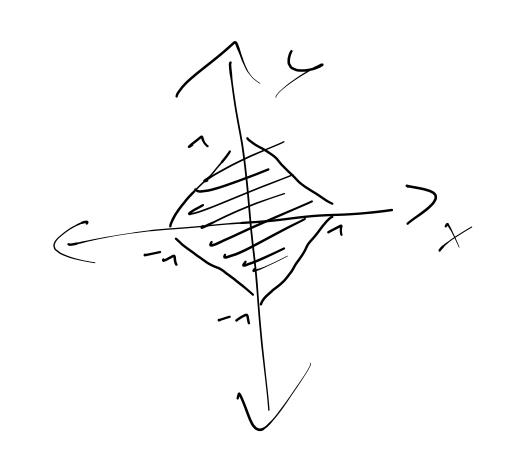
\includegraphics[width=8cm]{4_9_a}
    \end{figure}
    \FloatBarrier

    \item $M_1 = \{ (x,y)^T \in \mathbb{R}^2 \mid x^2 + y^2 > 1 \}$
    \begin{figure}[htbp]
        \centering
        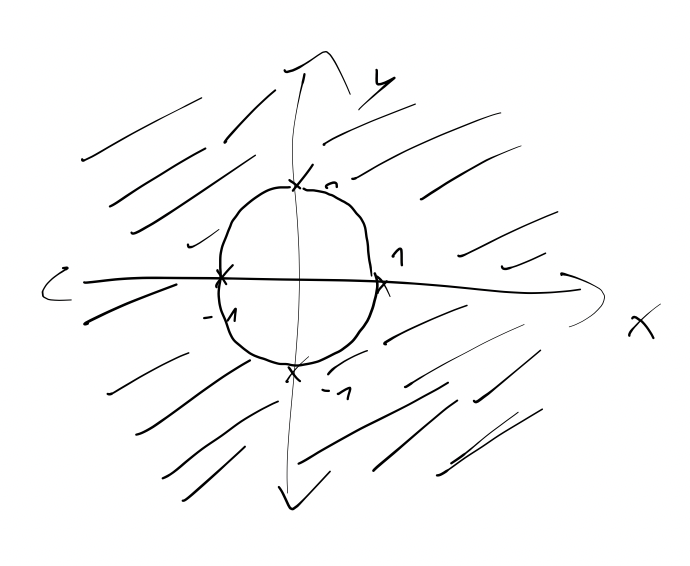
\includegraphics[width=8cm]{4_9_b}
    \end{figure}
    \FloatBarrier
    
    \item $M_1 = \{ (x,y)^T \in \mathbb{R}^2 \mid \max\{x,y\} \leq 1 \}$
    \begin{figure}[htbp]
        \centering
        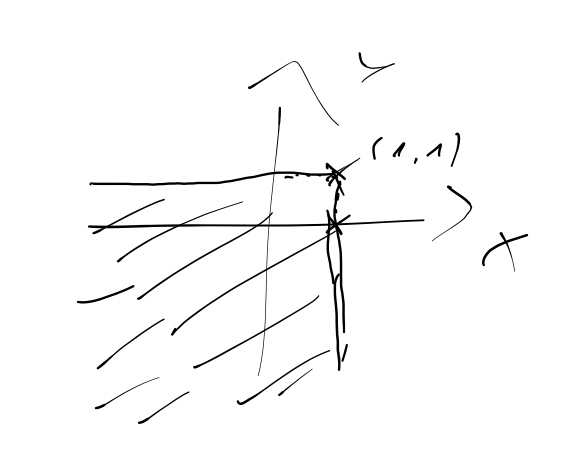
\includegraphics[width=8cm]{4_9_c}
    \end{figure}
    \FloatBarrier
\end{enumerate}

\subsection{Aufgabe 4.10}
% Hier eure Lösung eingeben
$$x_0 \in \mathbb{R} \text{, } A(x_0) \text{ gilt für } x < x_0$$
\begin{enumerate}[a)]
    \item $x =\frac{1}{2}x_0$ - gilt nicht, da $x_0$ negativ sein könnte
    \item $x =x_0 - 3$ - gilt nicht, da $x_0 - 3 < x_0$
    \item $y^2 < x_0$, bzw. $-\sqrt{x_0} < y < +\sqrt{x_0}$ für $x_0 \geq 0$. Wenn $x_0 < 0$ ist, existiert ein solches reelles $y$ nicht.
    \item \begin{align}
        \abs{y+2} &< x_0 \\
        y+2 > 0 &\vee y+2 < 0 \\
        y > -2 &\vee y < -2 \\
        \\
        y+2 < x_0 &\vee y+2 > x_0 \\
        y < x_0 -2 &\vee y > x_0 -2 \\
        \mathbb{L}_1 = ]-2,x_0 -2[ &\vee \mathbb{L}_2 = ]x_0-2, -2[
    \end{align}
    Es existiert kein $x_0$, für das beide Bedingungen erfüllt sind.
    Für $x_0 < 0$ gilt $\mathbb{L} = \mathbb{L}_2$ und andersherum.
\end{enumerate}

\subsection{Aufgabe 4.11}
% Hier eure Lösung eingeben
$$\abs{x^2 - 9} < \abs{x-1}$$
\begin{itemize}
    \item Fall 1: $x-1 > 0 \Leftrightarrow x > 1$\begin{align}
        \abs{x^2 - 9} &< x-1 
    \end{align}
    \item Fall 1.1: $x^2-9 > 0 \Leftrightarrow -3 > x > 3$\begin{align}
        x^2 - 9 &< x - 1 \\
        x^2 - x - 8 &< 0 \\
        (x-\frac{1}{2})^2 &< \frac{33}{4}
    \end{align}
    \item Fall 1.1.1: $x-\frac{1}{2} > 0 \Leftrightarrow x > \frac{1}{2}$\begin{align}
        x-\frac{1}{2} &< \frac{\sqrt{33}}{2} \\
        x &< \frac{1}{2} + \frac{\sqrt{33}}{2} \approx 3.37
        \Rightarrow \mathbb{L}_{1.1.1} = (\frac{1}{2}, 3.37)
    \end{align}
    \item Fall 1.1.2: $x-\frac{1}{2} \leq 0 \Leftrightarrow x \leq \frac{1}{2}$\begin{align}
        x-\frac{1}{2} > -\frac{\sqrt{33}}{2} \\
        x > \frac{1}{2} - \frac{\sqrt{33}}{2} \approx -2.37 \\
        \Rightarrow \mathbb{L}_{1.1.2} = (-2.37,\frac{1}{2}] \\
        \Rightarrow \mathbb{L}_{1.1} = (3, 3.37)
    \end{align}
    \item Fall 1.2: $x^2-9 \leq 0 \Leftrightarrow -3 \leq x \leq 3$\begin{align}
        x^2 - 9 &> 1-x \\
        x^2 + x -10 &> 0 \\
        (x+\frac{1}{2})^2 -\frac{41}{4} &> 0
    \end{align}
    \item Fall 1.2.1: $x+\frac{1}{2} > 0 \Leftrightarrow x > -\frac{1}{2}$\begin{align}
        x > -\frac{1}{2}+\frac{\sqrt{41}}{2} \approx 2.7
    \end{align}
    \item Fall 1.2.2: $x+\frac{1}{2} \leq 0 \Leftrightarrow x \leq -\frac{1}{2}$\begin{align}
        x < -\frac{1}{2}-\frac{\sqrt{41}}{2} \approx -3.7 \\
        \Rightarrow \mathbb{L}_{1.2} = (2.7, 3] \\
        \Rightarrow \mathbb{L}_{1} = (2.7, 3.37)
    \end{align}

    \item Fall 2: $x-1 \leq 0 \Leftrightarrow x \leq 1$\begin{align}
        \abs{x^2 - 9} &< 1-x
    \end{align}
    \item Fall 2.1: $x^2-9 > 0 \Leftrightarrow -3 > x > 3$\begin{align}
        x^2 - 9 &< 1 - x \\
        x^2 + x - 10 &< 0 \\
        (x+\frac{1}{2})^2 &< \frac{41}{4}
    \end{align}
    \item Fall 2.1.1: $x+\frac{1}{2} > 0 \Leftrightarrow x > -\frac{1}{2}$\begin{align}
        x+\frac{1}{2} &< \frac{\sqrt{41}}{2} \\
        x &< -\frac{1}{2} + \frac{\sqrt{41}}{2} \approx 2.7
    \end{align}
    \item Fall 2.1.2: $x+\frac{1}{2} \leq 0 \Leftrightarrow x \leq -\frac{1}{2}$\begin{align}
        x+\frac{1}{2} &> -\frac{\sqrt{41}}{2}\\
        x &> -\frac{1}{2} - \frac{\sqrt{41}}{2} \approx -3.7
        \Rightarrow \mathbb{L}_{2.1} = (-3.7,-3]
    \end{align}
    \item Fall 2.2: $x^2-9 \leq 0 \Leftrightarrow -3 \leq x \leq 3$\begin{align}
        x^2 - 9 &< x-1 \\
        x^2 - x -8 &< 0 \\
        (x-\frac{1}{2})^2 -\frac{33}{4} &> 0
    \end{align}
    \item Fall 2.2.1: $x-\frac{1}{2} > 0 \Leftrightarrow x > \frac{1}{2}$\begin{align}
        x > \frac{1}{2}+\frac{\sqrt{33}}{2} \approx 3.37
    \end{align}
    \item Fall 2.2.2: $x-\frac{1}{2} \leq 0 \Leftrightarrow x \leq \frac{1}{2}$\begin{align}
        x < \frac{1}{2}-\frac{\sqrt{33}}{2} \approx -2.37 \\
        \Rightarrow \mathbb{L}_{2.2} = [-3,-2.37)
        \Rightarrow \mathbb{L}_{2} = (-3.7,-2.37)
        \Rightarrow \mathbb{L} = (-3.7,-2.37) \cup (2.37,3.37)
    \end{align}


\end{itemize}

\subsection{Aufgabe 4.12}
% Hier eure Lösung eingeben
\begin{align}
    (ab + cd)^2 &\leq (a^2 + c^2)(b^2 + d^2) \\
    (ab)^2 + (cd)^2 + 2abcd &\leq (ab)^2 + (ad)^2 + (cb^2) + (cd)^2 \\
    2abcd &\leq (ad)^2 + (cb)^2 \text{, mit } ad = x \text{ und } cb = y\\
    2xy &\leq x^2 + y^2 \\
    0 &\leq x^2-2xy+y^2 \\
    0 &\leq (x-y)^2 \text{, das ist wahr}
\end{align}
\end{document}